\documentclass{article}
\usepackage{enumerate}
\usepackage{color}
\usepackage{graphicx}
\usepackage{amsmath}
\usepackage{geometry}
\usepackage{setspace}
\usepackage{minted}
\geometry{left=2.54cm,right=2.54cm,top=2.54cm,bottom=2.54cm}
\begin{document}
\begin{spacing}{2.0}
\vspace*{0.25cm}
\hrulefill
\thispagestyle{empty}
\begin{center}
\begin{large}
\sc{UM--SJTU Joint Institute \vspace{0.3em} \\ Introduction to Operating Systems \\ (VE482)}
\end{large}

\hrulefill


\vspace*{5cm}
\begin{Large}
\sc{Homework 2}
\end{Large}
\vspace{2em}
\end{center}
\vfill

\begin{table}[h!]
\flushleft
\begin{tabular}{lll}
Name: Yu Xiao \hspace*{2em}&
ID: 518021910696 \hspace*{2em}\\

Date: Oct 2, 2021
\end{tabular}
\end{table}
\end{spacing}

\hfill

\newpage

\noindent\textbf{Ex.1} -- \textit{MultiProgramming}
\begin{enumerate}
\item
The probability for $n$ processes to be waiting at the same time is $p^n$. \\
The CPU utilisation is $1-p^n$.
\item
The curve representing CPU utilisation with different $p$ is shown below.
\begin{figure}[h]
\centering
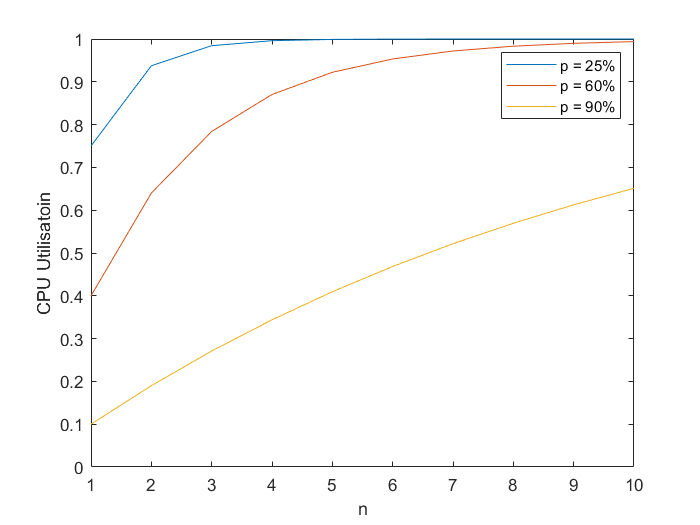
\includegraphics[width=0.8\linewidth]{VE482_h2_Ex1_2.png}
\end{figure}
\item
\begin{enumerate}[a)]
\item
After loaded the light operating system, we know that
$$\lfloor (256-96)\div 48\rfloor = 3$$
Therefore, $3$ processes can be stored simultaneously in memory.
\item
From previous question, we know that the CPU utilisation can be calculated by
$$1-0.9^3=27.1\%$$
Therefore, the CPU utilisation in this case is $27.1\%$.
\item
If 256 MB is added, $\lfloor (512-96)\div 48\rfloor = 8$ processes can be stored simultaneously in memory, the CPU utilisation will be $1-0.9^8\approx56.95\%$, which increases by $(56.95\% \div 2)-27.1\% =29.85\%$ per 256 MB.\\
If 512 MB is added, $\lfloor (768-96)\div 48\rfloor = 14$ processes can be stored simultaneously in memory, the CPU utilisation will be $1-0.9^14\approx77.12\%$, which decreases by $\vert(77.12\% \div 3)-27.1\%\vert =1.39\%$ per 256 MB.\\
If 1024 MB is added, $\lfloor (1280-96)\div 48\rfloor = 24$ processes can be stored simultaneously in memory, the CPU utilisation will be $1-0.9^24\approx92.02\%$, which decreases by $\vert(92.02\% \div 5)-27.1\%\vert = 8.7\%$.\\
As a result, adding 256 MB will be the most beneficial and worth the investment.
\end{enumerate}
\end{enumerate}

\noindent\textbf{Ex.2} -- \textit{Keymap in Minix 3}\\
In \mintinline{shell}{/usr/src/servers/is/dump.c},
\end{document}